\documentclass[border=10pt]{standalone}

\usepackage{tikz}
\usepackage{tikzsymbols}
\usetikzlibrary{calc,patterns,shapes.geometric}

\def\centerarc[#1](#2)(#3:#4:#5){\draw[#1] ($(#2)+({#5*cos(#3)},{#5*sin(#3)})$) arc (#3:#4:#5);}

\begin{document}
	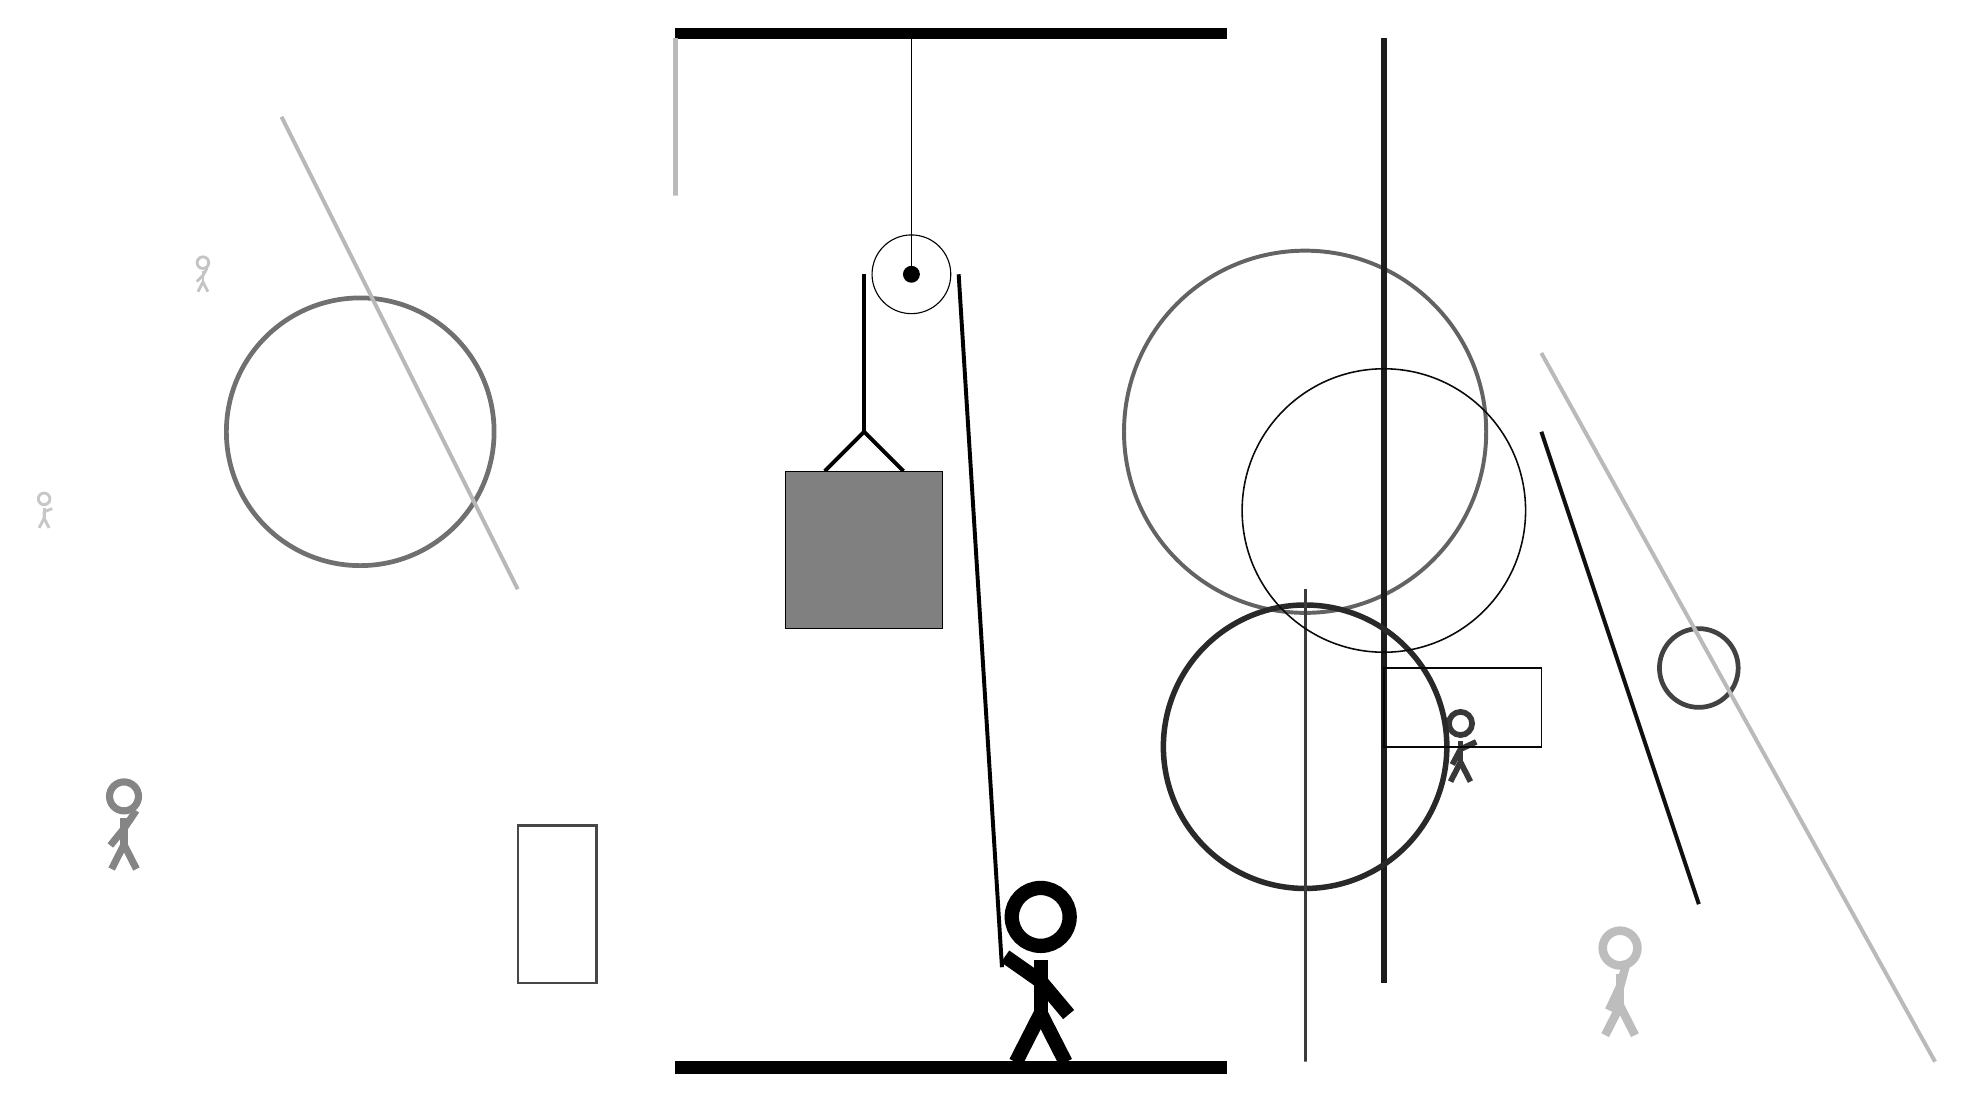
\begin{tikzpicture}
		%%%%% START %%%%%
		
		\draw[fill=black] (-2, 10) rectangle (5, 10.125);
		
		\draw (1, 7) circle (0.5);
		\draw[fill=black] (1, 7) circle (0.1);
		\draw (1, 10) -- (1, 7);
		
		\draw[line width=0.5mm] (-0.1, 4.5) -- (0.4, 5.0) -- (0.9, 4.5);
		\draw[fill=black!50] (-0.6, 4.5) rectangle (1.4, 2.5);
		
		\draw[line width=0.5mm] (0.4, 7) -- (0.4, 5.0);
		\centerarc[line width=0.5mm](1, 7)(0:180:0.6);
		\draw[line width=0.5mm](1.6, 7) -- (2.15, -1.8);
		
		\node[line width=0.5mm, color=black!23] at (-8, 7) {\Strichmaxerl[2][45][61]};
		
		\node[line width=0.4mm, color=black!78] at (8, 1) {\Strichmaxerl[4][62][25]};
		\draw [line width=0.5mm, color=black!61](6, 5) circle (2.3);
		\draw [line width=0.6mm, color=black!56](-6, 5) circle (1.7);
		\draw [line width=0.6mm, color=black!74](11, 2) circle (0.5);
		\node[line width=0.5mm, color=black!48] at (-9, 0) {\Strichmaxerl[5][51][56]};
		
		\draw[line width=0.7mm, color=black!89] (7, -2) rectangle (7, 10);
		\draw[line width=0.5mm, color=black!94](9, 5) -- (11, -1);
		\draw [line width=0.7mm, color=black!84](6, 1) circle (1.8);
		\node[line width=0.5mm, color=black!26] at (10, -2) {\Strichmaxerl[6][65][75]};
		
		\draw[line width=0.5mm, color=black!28](-7, 9) -- (-4, 3);
		\draw[line width=0.3mm, color=black!72] (-4, -2) rectangle (-3, 0);
		\draw[line width=0.4mm, color=black!77] (6, 3) rectangle (6, -3);
		
		\draw [line width=0.2mm, color=black!96](7, 4) circle (1.8);
		\draw[line width=0.6mm, color=black!27] (-2, 8) rectangle (-2, 10);
		\draw[line width=0.2mm, color=black!97] (7, 1) rectangle (9, 2);
		
		\node[line width=0.7mm, color=black!22] at (-10, 4) {\Strichmaxerl[2][89][21]};
		\draw[line width=0.5mm, color=black!27](9, 6) -- (14, -3);
		
		\node at (2.6, -1.9) {\Strichmaxerl[10][-35][-50]};
		
		\draw[fill=black] (-2, -3) rectangle (5, -3.15);
		
		%%%%% END %%%%%
	\end{tikzpicture}
\end{document}